\section{Animations and Lights}
Following the MVC pattern, animations' and lights' creation and management takes place in the \textit{View/ViewMediator} and \textit{Control} classes related to the respective \textit{Model}.\\
By the following subsections there will be described with more detail the code, where necessary, and the execution related to the most important components of the project.
\subsection{Turret}
The turret is the most complex object and obviously their parts are animated separately:
\begin{itemize}
\item \textbf{Supporto: } it is the parent of all components, in particular it rotates along the y-axis following the mouse x-coordinates.
\item \textbf{Bracci: } they rotate on the x-axis following the mouse y-coordinates.
\item \textbf{Canne: } their animation is a translation on z-axis, it also has a color animation indicating the overheating.
\end{itemize}
\begin{figure}[h!]
\begin{center}
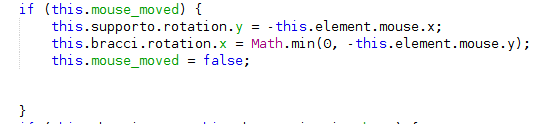
\includegraphics[scale=0.35]{images/supporto_bracci_anim.png}
\caption{The code in charge of animate \textit{Supporto} and \textit{Bracci}}
\end{center}
\end{figure}
\subsection{Bullet}
The TurretMediator builds also a Plane far away in front of the camera that someway indicates the Far into the frustum, covering all the background.
On mouse down event for every created bullet, the system calculates the intersection point with mouse coordinates and the plane in 3D space and passes it to the BulletMediator throught the related model. Once the BulletMediator launches his makeObject3D method also builds two lines starting from the turret and going to the given point. On each iteration of the render frame the bullet translate along the line for a bigger step depending on the bullet mediator's speed with the THREEJS method \textit{at}.
\subsection{Storms implementations}
As described before, both the Storms share a common behaviour, related on how the two game modes keep active the interactions between the enemies, the environment and the player's actions.\\
As we can inspect from the code of both the Controller classes regarding the \textit{onGame} function that is used to execute the current frame animation, both the game modes can be subdivided in the following parts:
\begin{itemize}
\item \textit{If statement} that checks whether a game-over status hasn't been already reached or the game isn't in pause, that also leads to the following actions:
\begin{itemize}
\item deployment, check and movement of the enemies under the rules of the actual Storm;
\item check whether a winning or a losing condition has been reached;
\item synchronize the \textit{UI} (User Interface) with the obtained data;
\end{itemize}
\item \textit{If statement} that checks if a reset have to be instantiated, making all enemies to return to their initial state and acting on the content of the UI.
\end{itemize}
\begin{figure}[h!]
\begin{center}
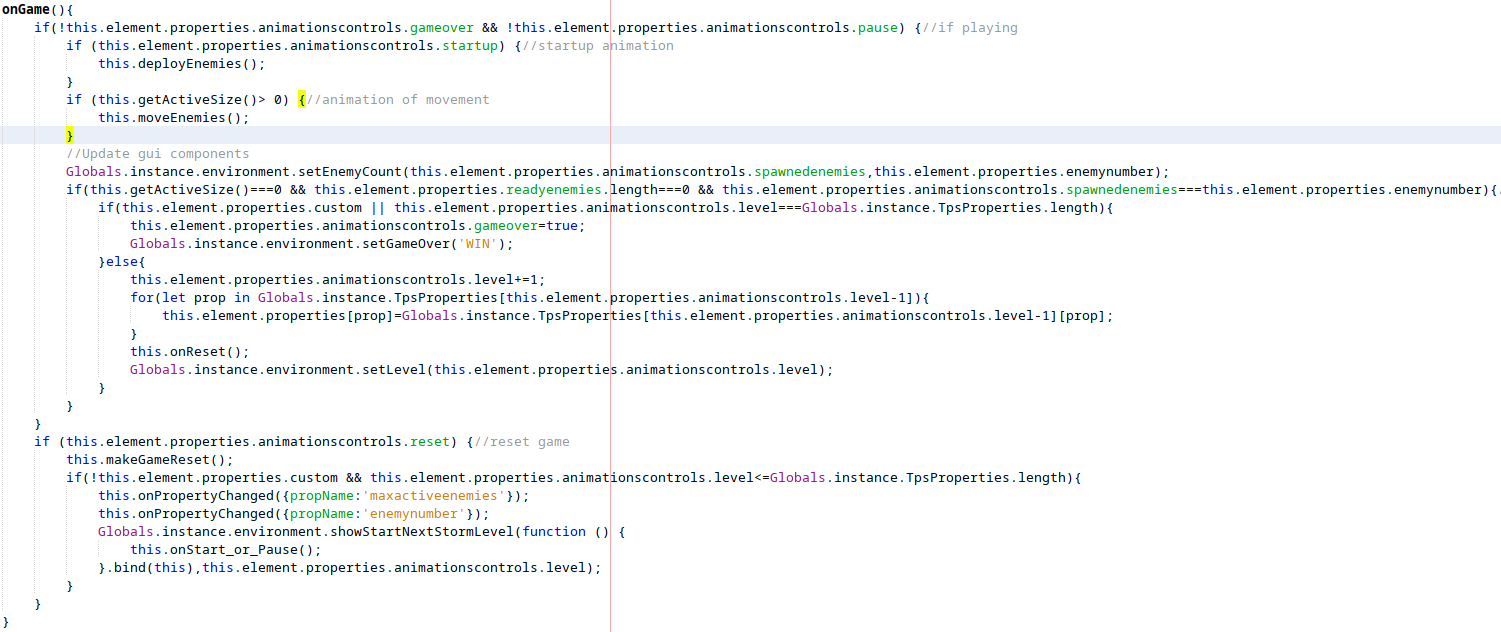
\includegraphics[scale=0.3]{images/onGame-code.png}
\caption{TPStorm render calculation function, from TpsController.js file.}
\end{center}
\end{figure}
There are also similar patterns of implementation regarding the type of mode that would be executed:
\begin{itemize}
\item \textit{Arcade mode}: the game can't reach the Win condition unless the final level has been beaten, otherwise forcing a soft-reset (not touching the score) at each wave;
\item \textit{Custom mode}: each Storm invokes the creation of a \textit{Gui} that allows the interaction of the player with the gaming scene acting on some parameters that subordinate the movements and the appearance of the enemies and also the light of the environment.
\end{itemize}
\begin{figure}[!h]
   \begin{minipage}{0.50\textwidth}
     \centering
     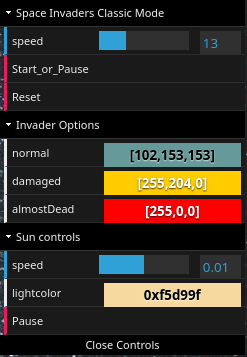
\includegraphics[scale=0.28]{images/StormGui.png}
     \caption{\small Storm GUI.}
   \end{minipage}\hfill
   \begin{minipage}{0.50\textwidth}
     \centering
     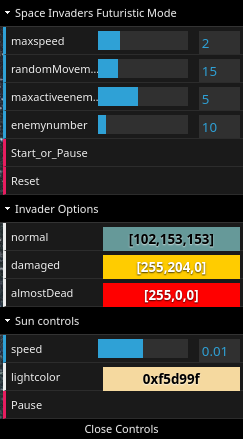
\includegraphics[scale=0.28]{images/TPStormGui.png}
     \caption{\small TPStorm GUI.}
   \end{minipage}
\end{figure}
In every mode the player wins only if all the enemies have been destroyed before a lose condition has been verified.\\
In the following subsections there will be described the peculiarities of each mode in the management of the invaders.

\subsubsection{Storm}
In the \textit{Classic mode} the enemies' group have to bounce from one corner of the screen remaining always visible to the player. Whenever a corner is trespassed by a spaceship, the direction of the horizontal movement is changed and all the enemies are pushed down by a certain amount of space. If, during the game execution, the enemies' number decreases their speed increases, making harder the elimination of the remaining spaceships. \\
When an enemy is destroyed it is put in an hidden position under the map in order to avoid a possible interference with the turret's shoots. It will return to its starting point only if a reset is called.\\
The player loses when an enemy reaches a fixed y that coincides with the ground in its position.
\begin{figure}[h!]
\begin{center}
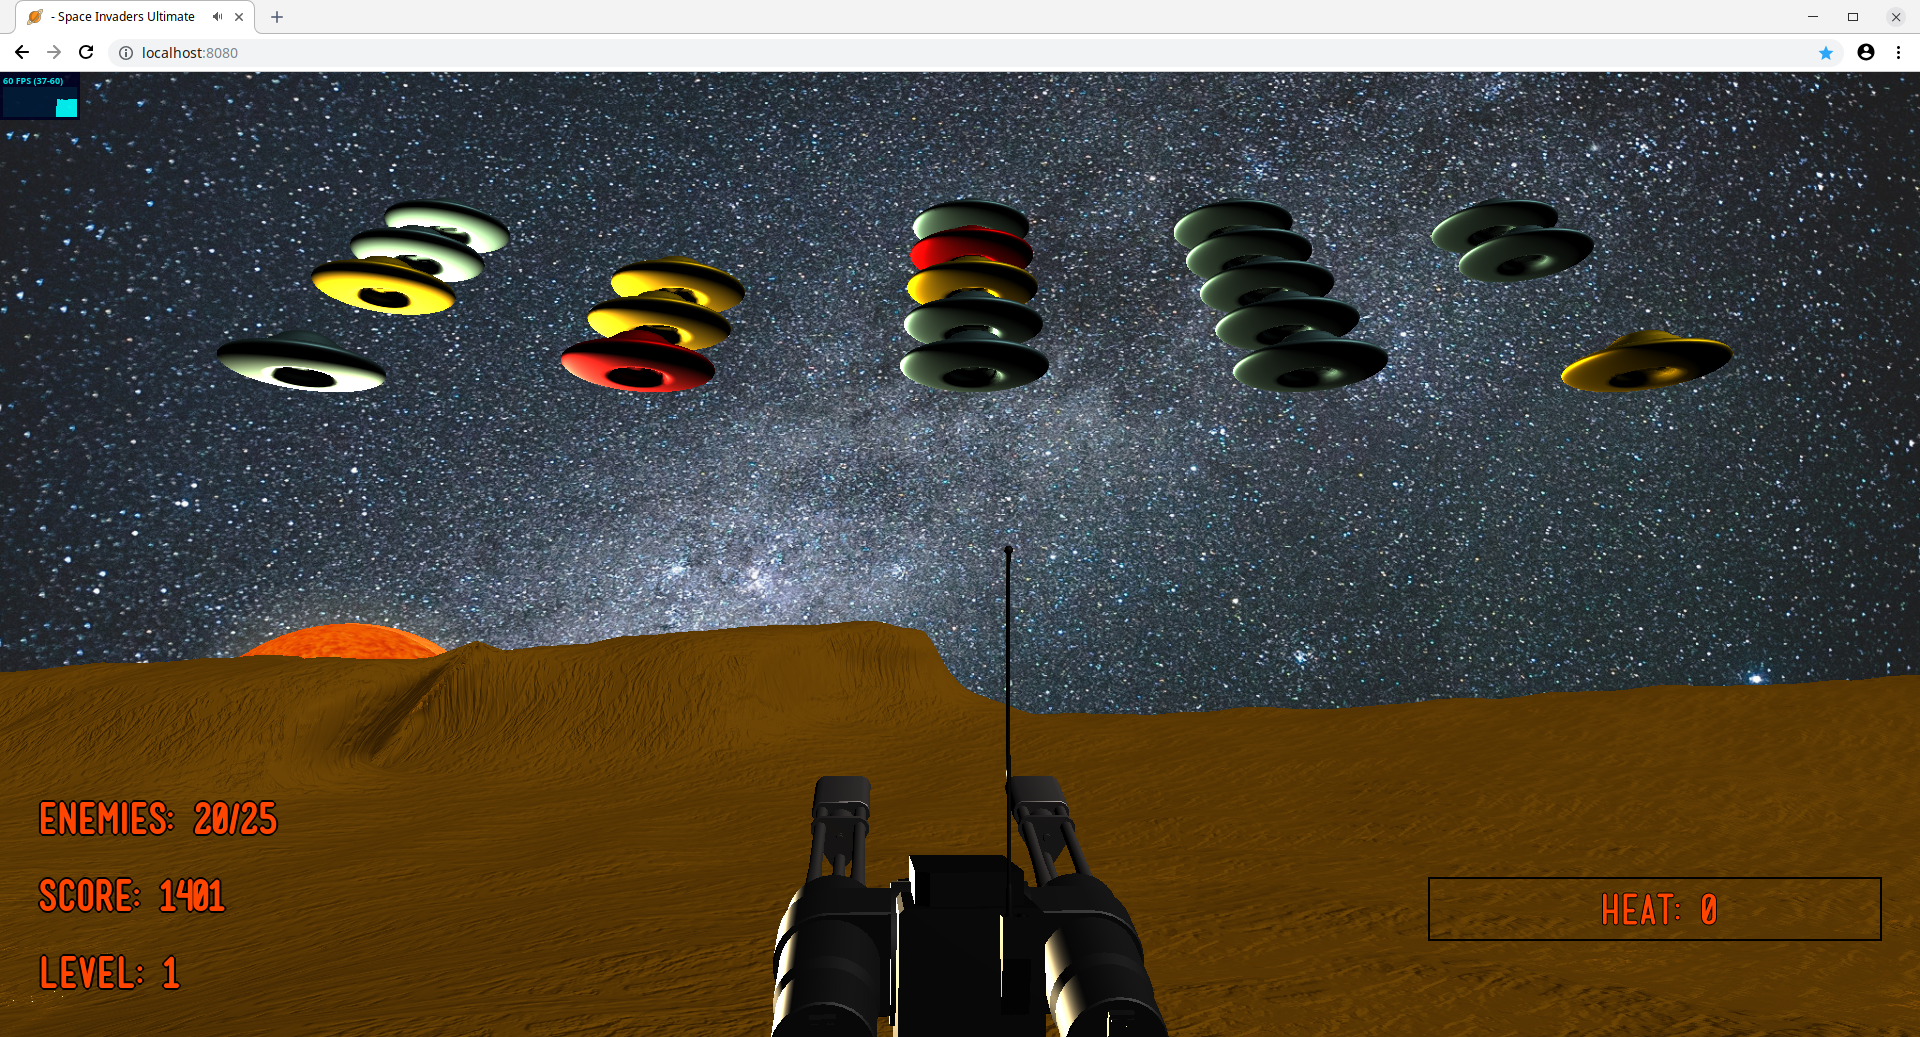
\includegraphics[scale=0.18]{images/onGoing_Storm.png}
\caption{Storm during a wave.}
\end{center}
\end{figure}
\subsubsection{TPStorm}
In the \textit{Futuristic mode}, as said before, each enemy is independent from another and starting from one of the two fixed spawning points it has to reach a random ending-point passing through a fixed number of random intermediate points. During all the execution the spaceship speed remains constant but results higher than the Classical's counterpart. Moreover in this mode the behaviour of the spaceships is perceived as less predictable by the player, so making higher the grade of challenge, especially when a lot of enemies are on the screen.\\
When an enemy is destroyed it is restored to its spawning-point and a new random ending-point is assigned to it. If another enemy is needed in order to complete the current wave then it is put in a ready-queue that allows a future \textit{respawn} as a new enemy.\\
As it can be easily assumed, the player loses when an enemy reaches its own assigned ending-point.
\begin{figure}[h!]
\begin{center}
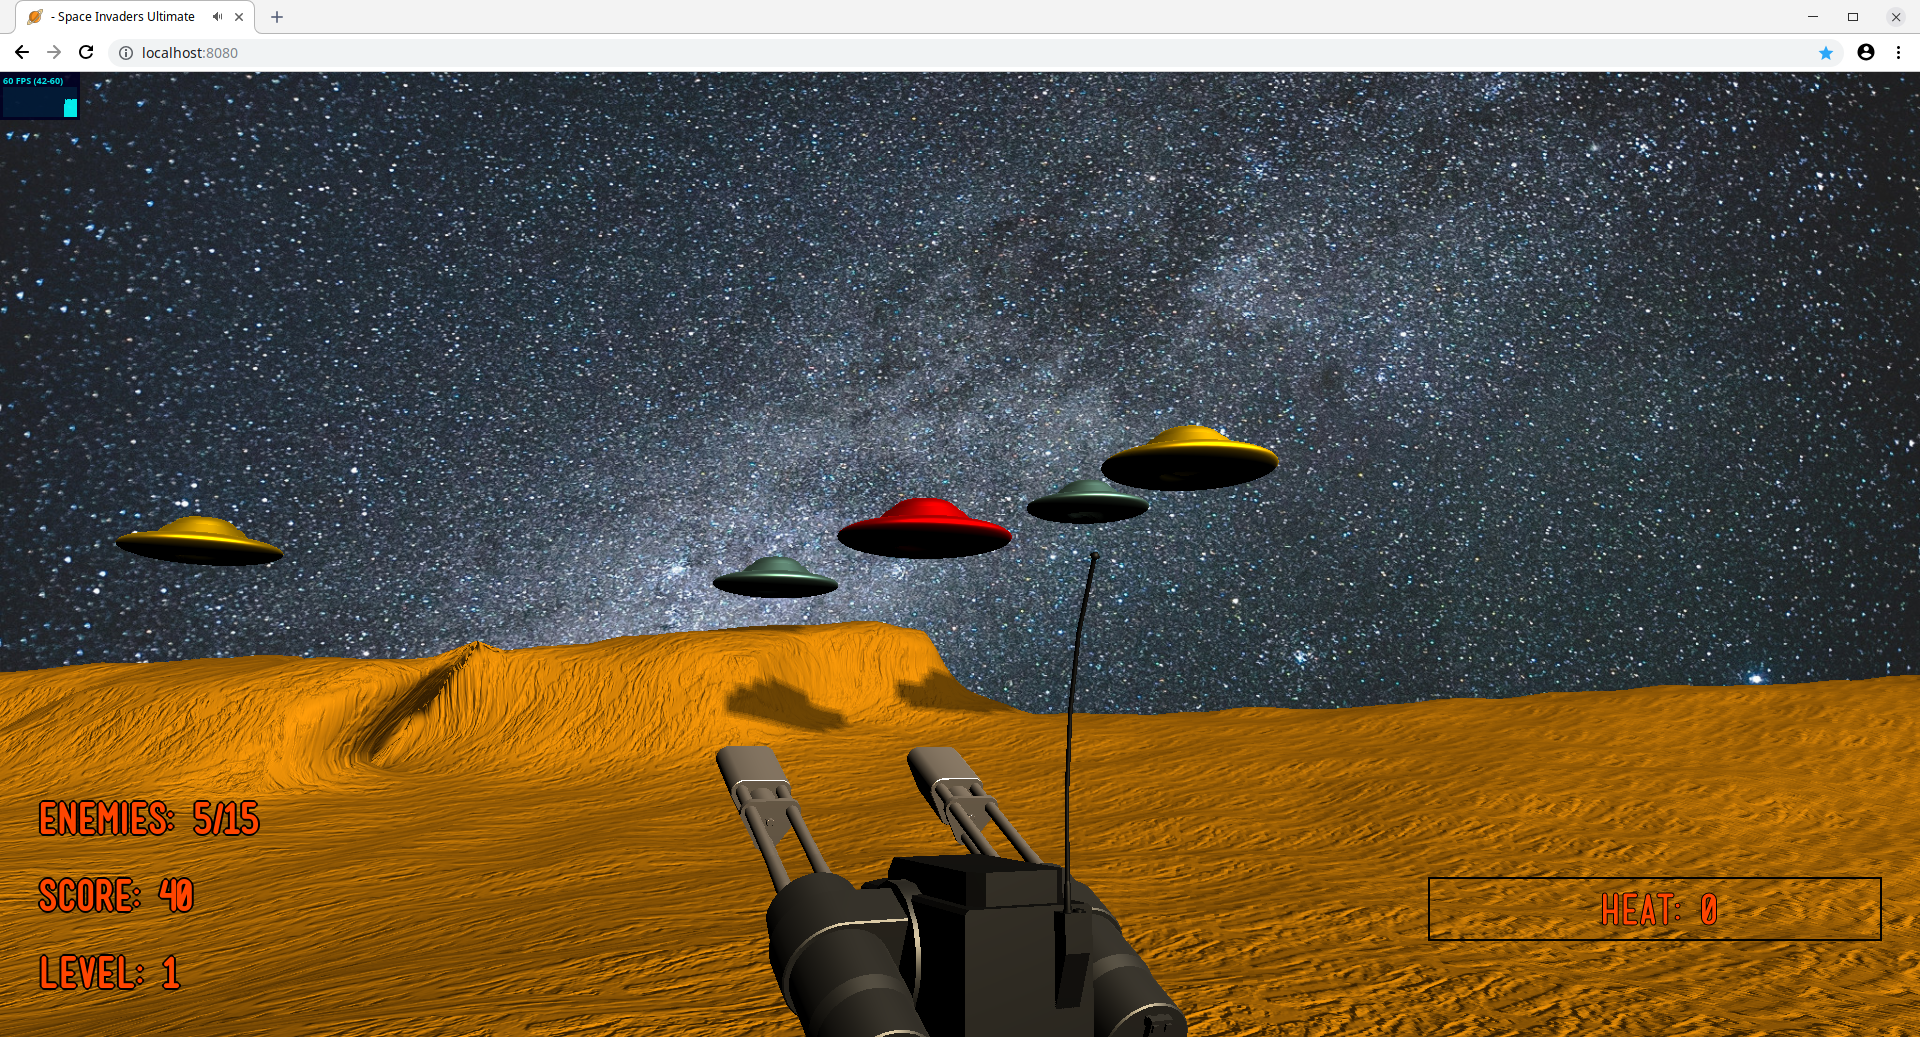
\includegraphics[scale=0.18]{images/onGoing_TPStorm.png}
\caption{TPStorm during a wave.}
\end{center}
\end{figure}

\subsubsection{Enemy}
The enemy is a single block model, so the animation is not as complicate as the turret one, anyway would be interesting to better know how it moves. First let define the movement it does:
\begin{enumerate}
\item Rolling
\item Explosion
\item Movement into the space
\end{enumerate}
The third one depends only to the storm, so in the next two paragraphs we'll focus only on the first two ones.
\paragraph{Rolling}: \\
After an hit the enemy rolls on the z-axis, following the rule of the \textbf{Underdamped Oscillator}

\begin{equation}
x = e^{-\gamma t}\alpha cos[\omega_1t-\alpha]
\end{equation}
The implementation differs from the rule just for a \textit{t} value that activates the roll only when it's less than the number of phases defined
\begin{figure}[h!]
\begin{center}
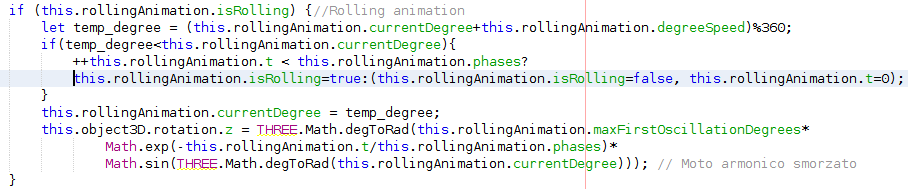
\includegraphics[scale=0.4]{images/rolling.png}
\caption{Implementation of Underdamped Oscillator's equation.}
\end{center}
\end{figure}

\paragraph{Explosion}
After the third hit the enemy explodes. The animation works on a second object that is hidden and overlapped to the living enemy. That object is a configurable set of THREE.Points that is created by the function \textit{explodeAnimation} which alsco creates an array of random directions (one per point) representing a random generated value between \textit{this.movementSpeed / 2} and \textit{-this.movementSpeed / 2} . During the explosion the rendering calls the function \textit{updateExplosion} increases/decreases the position on every axis by the generated direction.
\begin{figure}[h!]
\begin{center}
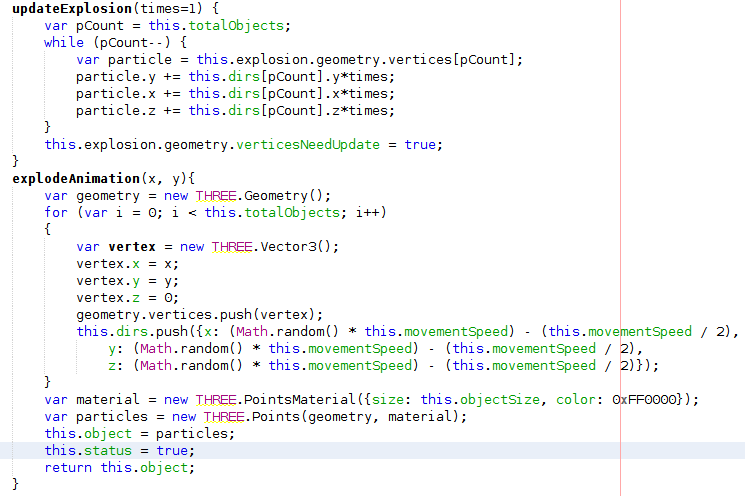
\includegraphics[scale=0.4]{images/explosion.png}
\caption{The code responsible for the explosion animation.}
\end{center}
\end{figure}
\newline
\subsection{Lights and Shading}
In the scene there have been introduced two sources of light:
\begin{itemize}
\item \textit{AmbientLight} that allows the presence of a minimum illumination in the scene also withouth a direct source of light;
\item \textit{PointLight} that is the main source of light that propagates in every direction and it's also responsible for the shadow casting and the shading effects on the objects.
\end{itemize}

In order to obtain a very dynamic effect that also changes during the course of game and the various waves the PointLight has been put as a child of a \textit{Sun} object (a textured sphere) that periodically orbits around the ground.\\
The source of light shares the same color of the moving star. During the execution of the various waves, it has been implemented that also the Sun changes its color according to the number of the current level. This allows the perception of different atmospheres during the continuation of the game, making each intermediate level even more different.\\
These types of variations are also possible and let free to the player in the Custom mode GUI.\\
Following to the Threejs documentation\cite(threejsdoc), the enabling of shadows to the objects of the scene takes only few lines of code, acting only on the \textit{THREE.renderer} object, on the \textit{light-source} and on the involved \textit{meshes}:
\begin{figure}[!h]
   \begin{minipage}{0.33\textwidth}
     \centering
     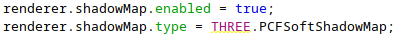
\includegraphics[scale=0.35]{images/renderer-shadow.png}
     \caption{\small Renderer settings.}
   \end{minipage}\hfill
   \begin{minipage}{0.33\textwidth}
     \centering
     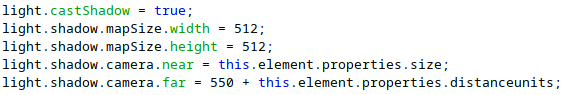
\includegraphics[scale=0.35]{images/light-shadow.png}
     \caption{\small Light settings.}
   \end{minipage}
   \begin{minipage}{0.33\textwidth}
     \centering
     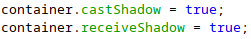
\includegraphics[scale=0.35]{images/object-shadow.png}
     \caption{\small Object settings.}
   \end{minipage}
\end{figure}